\vspace{-0.7\baselineskip}
\section{Geometry estimation with edge-aware depth-normal consistency}
\label{sec:approach}
\vspace{-0.3\baselineskip}

In our scenario, given target image $I$, we aim to learn to estimate both depth and normal simultaneously. Formally, let $N$ be the predicted normal from our model, we embed it into the training pipeline and make it a stronger regularization for estimating depth $D$, which help to train more robust model.

\vspace{-0.5\baselineskip}
\subsection{Depth and normal orthogonality.}
\label{sub:depth_and_normal_orthogonality}
\vspace{-0.3\baselineskip}

In reconstruction, depth and normal are two strongly correlated information, which usually follow locally linear orthogonality correlation. Formally, for each pixel $x_i$, such a correlation can be written as a quadratic minimization for a set of linear equations, either given depth or normal,
\begin{align}
\label{eq:orthognal}
&\scr{L}_{x_i}(D, N) = ||[\cdots,\omega_{ji}(\phi(x_j) - \phi(x_i)), \cdots]^T  N(x_i)||^2, \nonumber \\
&~\text{where~} \phi(x) = D(x)\ve{K}^{-1}h(x), \text{~} \|N(x_i)\|_2 = 1, \nonumber\\
&~\text{~~~~~~~~} \omega_{ji} > 0 \text{~~if~~} x_j \in \hua{N}(x_i)
\end{align}
where $\scr{N}(x_i)$ is a set of predefined neighborhood pixels of $x_i$, and $N(x_i)$ is a $3 \times 1$ vector. $\phi(x)$ is back projected 3D point from 2D coordinate $x$. $\phi(x_j) - \phi(x_i)$ is a difference vector in 3D, and $\omega_{ji}$ is used to weight the linear equation for pixel $x_j$ which we will elaborate later.

However, as introduced in Sec. \ref{sec:related}, most supervised works try to predict the two information independently without considering their correlations, SURGE~\cite{peng2016depth} proposes to apply the consistency by a post CRF processing only over large planar regions. In our case, we enforce the consistency over the full image, and directly applied to network output, which better benefits the model learning. Specifically, to model their consistency, we developed two layers by solving \equref{eq:orthognal}, \ie depth to normal layer and normal to depth layer. 

\textbf{Infer normals from depths.} 
\label{chap:d2n}
Given a depth map $D$, for each point $x_i$, in order to get $N(x_i)$ by solving \equref{eq:orthognal}, we need to firstly define $\hua{N}(x_i)$ and $\omega_{ji}$, and then solve the set of linear equations. To deal with the first issue, we choose using the 8-neighbor convention to compute normal directions, which considerably more robust than 4-neighbor convention. 
However, it is not always good to equally weight all pixels due to depth discontinuity or dramatic normal changes may occur nearby. Thus, for computing $\omega_{ji}$, we set it large neighboring pixels $x_j$ having similar color with $x_i$, while smaller otherwise. Formally, $\omega_{ji} = \exp\{-\alpha|I(x_j) - I(x_i)|\}$ and $\alpha = 0.1$ in our case. 

For minimizing \equref{eq:orthognal}, one may apply a standard singular value decomposition (SVD) to obtain the solution. However, in our case, we want to embed such an operation in the network training and back-propagate the gradient respect to input depth. SVD is computationally non-efficient for back-propagation. Thus, we choose to use mean cross-product to approximate the minimization~\cite{jia2006using}, which is simpler and more efficient. 
Specifically, from the 8 neighbor pixels around $x_i = [m, n]$, we split them to a set of 4 pairs, where each pair of pixels is perpendicular at 2D \wrt $x_i$, and in a counter clock-wise order, \ie $\hua{P}(x_i) = \{([m-1, n], [m, n+1]), \cdot, ([m+1, n-1], [m-1, n-1])\}$. 
Then, for each pair, cross product of their difference vector \wrt $x_i$ is computed, and the mean of computed vector is assign to the normal direction of $x_i$. Formally, the solver for normal is written as, 
\begin{align}
\label{eq:cross}
&\ve{n} = \sum_{p\in\hua{P}}(\omega_{p_{0}, x_i}(\phi(p_{0}) - \phi(x_i)) \times \omega_{p_{1}, x_i}(\phi(p_{1}) - \phi(x_i))), \nonumber \\
&N(x_i) = \ve{n} / \|\ve{n}\|_2
\end{align}
The process of calculating the normal direction using one pair of pixels is in Fig. \ref{fig:d2n}. 

%for each $q\in\theta(p)$, $R_q$ satisfies $(q-p)\cdot(r-p) = 0, \quad r \in R_q$.
% The normal direction of each point is computed based on the neighboring points after projecting to 3D space. The process of calculating normal direction of point $p$ is shown in Figure \ref{fig:d2n}. $\theta(p)$ is a set of neighboring (8) points of $p$. 
% Take point $q \in \theta(p)$ for example. $R_{q}$ is a set of points that satisfy the requirement: when projecting to 3D space, for $\hat{q} \in \hat{\theta}(p)$ and for $\hat{r} \in \hat{R}_{q}$, $(\hat(q)-\hat(p) \cdot (\hat{r} - \hat(p)) \neq 0)$. Symbols with hat represent corresponding points in 3D space. Theoretically, the cross-product of any two non-collinear (in 3D space) vectors connecting $\hat{p}$ and $\hat{\theta}(p)$ is the normal direction $N(p)$. To reduce the possiblity that the two vectors being collinear in 3D space, we require the vectors to be perpendicular when projected in 2D plane. The normal directions are averaged when iterating $q \in \theta(p)$, and then $l_2$ normalized to make it a unit vector. The normal direction is calculated as:

\begin{figure}
\centering
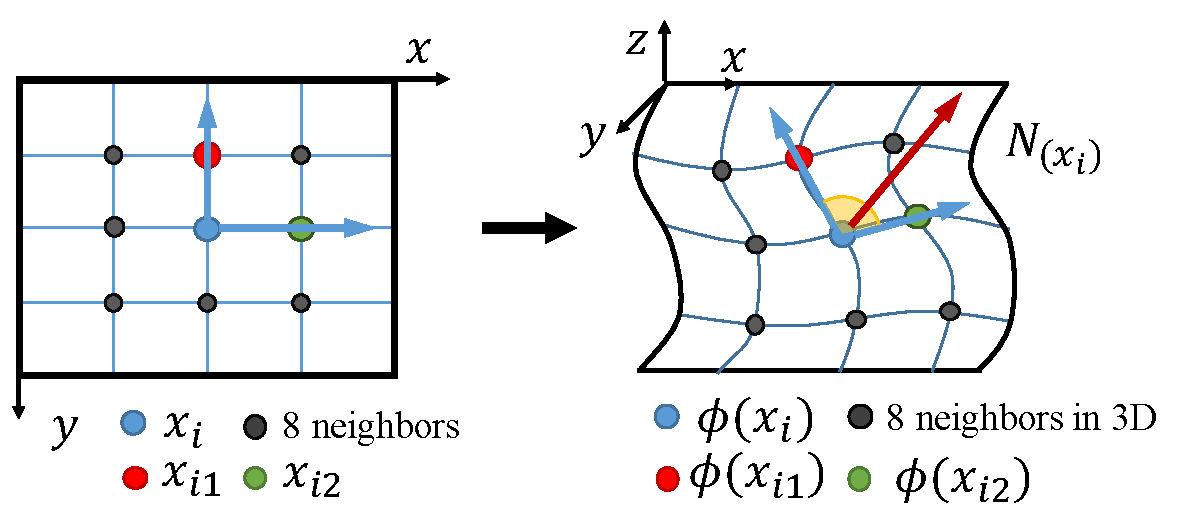
\includegraphics[width=0.5\textwidth]{figures/d2n.pdf}
\caption{Illustration of computing normal base on a pair of neighboring pixels. $x_i, x_{i1}, x_{i2}$ are 2D points, and 
$\phi(x_i), \phi(x_{i1}), \phi(x_{i2})$ are corresponding points projected to 3D space. 
The normal direction $N(x_i)$ is computed with cross product between $\phi(x_{i1}) - \phi(x_i)$ and $\phi(x_{i2}) - \phi(x_i)$.}
\vspace{-0.7\baselineskip}
\label{fig:d2n}
\end{figure}

\textbf{Expect depths from normals.} 
Due to the fact that we do not have ground truth normal for supervision, it is necessary to recover depth from normal to receive the supervision from photometric error as discussed in Sec.~\ref{sec:preliminaries}.
To recover depth, given normal map $N$, we still need to solve \equref{eq:orthognal}. However, there is no unique solution. Thus, for simplicity, we provide an initial depth map $D_o$ as input, which might lack normal smoothness, \eg depth map from network output. Then, given $D_o(x_i)$, the depth solution for neighboring pixel is unique and can be easily computed. Formally, let $D_e(x_j | x_i) = \psi(D_o(x_i), N(x_i))$ be the expected depth value calculated for a neighbor pixel $x_j$ \wrt $x_i$. 
However, when computing over the full image, we still need to solve 8 equations jointly for each pixel from its 8 neighbors. Finally, by minimum square estimation, the solution for the expected depth value is,
\begin{align}
\label{eq:depth}
D_n(x_j) = \sum_{i\in\hua{N}}\hat{\omega}_{ij}D_e(x_j | x_i), \text{~~}
\hat{\omega}_{ij} = \omega_{ij} / \sum_i{\omega_{ij}}
\end{align}

 %ormal2depth layer takes depth map and normal map as input and outputs a ``shifted" depth map. Take Figure \ref{fig:d2n} for example, the depth values of points $\theta(p)$ can be calcuated with the depth and normal direction of point $p$ known. From the calculation of normal direction, $(\hat{p} - \hat{q}) \cdot N(p) = 0$. When projecting points from 2D plane to 3D space, $\hat{p} = K^{-1}p$. $\hat{p} = (\hat{x}_p),\hat{y}_p,\hat{z}_p$, $p = (x_p, y_p, z_p)$ is a homogeneous 2D point and $z_p$ is the depth value of point $p$. $K^{-1}$ is the inverse of intrinsic matrix, which is determined by the camera. In linear the equation between depth and normal direction, $(K^{-1}(x_p, y_p, z_p) - K^{-1}(x_q, y_q, z_q))\cdot N(p) = 0, q\in\theta(p)$, the only unknown $z_q$, \ie  depth value of point $q$, has a unique solution. 

%As there are multiple points in the set $\theta(p)$, multiple depth maps can be recovered corresponding to each point $q \in \theta(p)$. In our pratice, the $\theta(p)$ includes 8 nearest points around point $p$. The 8 depth maps are weighted averaged to produce a reasonable depth output. As depth and normal discontinuity often happens where image gradients are large, similar to using image gradient in smoothness loss term, the image gradients are also calculated as weights to determine how much of each depth map contribute to final output. The output depth map is calculated as:
% $$z_p = \sum_{\theta(p)}z_q\frac{e^{(-\alpha|\partial_{\overrightarrow{p-q}}I_p|)}}{\sum_{\theta(p)}e^{(-\alpha|\partial_{\overrightarrow{p-q}}I_p|)}}, q\in\theta(p)$$
% In which, $\partial_{|\overrightarrow{p-q}}I_p|$ is the image gradient value along the $\overrightarrow{p-q}$ direction.
\vspace{-0.7\baselineskip}
\subsection{Training losses}
\label{sub:training_losses}
\vspace{-0.3\baselineskip}

In this section, we describe our training strategy. In order to supervise both the depth and normal representations, we can directly applied the loss in \equref{eqn:full} by replacing the output from network $D_o$ with the output after normal to depth layer $D_n$ to train the model. We show in our experiments (\secref{sec:experiments}, by doing this, we outperform the previous state-of-the-art by around 10$\%$ in depth estimation using the same network architecture.

Additionally, with normal representation, we additionally require smoothness over neighboring normal values, which provides high order interactive between pixels. Formally, the smoothness for normal haves the same form as $\scr{L}_{s}$ in \equref{eqn:regular}, while we apply the first order gradient, \ie $\scr{L}_{s}(N, 1)$. 

Last but not the least, matching corresponding pixels between frames is another central factor to find correct geometry. Additional to photometric error from matching pixel colors, matching image gradient is more robust to lighting variations, which was frequently applied in computing optical flow~\cite{li2017pyramidal}. 
In our case, we compute a gradient map of the target image and synthesized target images, and include the gradient matching error to our loss function. Formally, the loss is represented as,
\begin{equation}
\label{equ:gradient}
\scr{L}_{g}(D_n, \hua{T}, \hua{M}) = \sum_{s=1}^{S}\sum_{x_t}\ve{M}_s(x_t)\|\nabla I_t(x_t) - \nabla \hat{I_s}(x_t)\|_1, \nonumber
\end{equation}
In our experimental section, we observe additional benefits by having this match, especially at indoor scenario, where colors are often homogeneous on walls.
In the future, we hope to investigate more in matching criteria such as with stronger descriptors like SIFT~\cite{liu2011sift} or higher level convolutional features.

In summary, our final learning loss for multi-scale learning is,
\begin{align}
\label{eq:full_loss}
&\scr{L}(\hua{D}, \hua{N}, \hua{T}, \hua{M}) = \scr{L}_{o}(\{D_{nl}\}, \hua{T}, \hua{M}) + \nonumber\\
&\text{~~~~~~~~~}\sum_l\{\lambda_g\scr{L}_{g}(D_{nl},\hua{T},\hua{M}) + \lambda_n\scr{L}_{s}(N_l, 1)\}
\end{align}
where $\hua{D} = \{D_{nl}\}$ and $\hua{N} = \{N_{l}\}$ are the set of depth maps and normal maps for the target view.

%Our intuition is to train a CNN that is capable of modeling the geometry consistency of a mostly rigid scene. To facilitate the learning of the network, we explicitly propose to model the constraint between depth and normal. The training samples of the framework consist of frame sequences captured by a monocular moving camera.normalsize

\textbf{Training the model.} For network architectures, similar to \cite{zhou2017unsupervised} and \cite{godard2016unsupervised}, we adopt the DispNet \cite{mayer2016large} architecture with skip connections as in \cite{zhou2017unsupervised}. All \textit{conv} layers are followed by a ReLU activation except for the top prediction layer. We train the network from scratch, since too many losses at beginning could be hard to optimize, we choose a two stage training strategy by first train the network with $\scr{L}_{o}$ with 5 epochs and then fine-tune it with the full loss for 1 epoch. We will provide ablation study of each term in our experiments.


% To model a reasonable geometrical consistency, we propose the overall objective function as in Equation \ref{equ:1}.
% \begin{equation}
% \label{equ:1}
% \begin{split}
% L(D, I, Rt, \lambda) = L_{warp}(D, I, Rt) + L_{smooth}(D, N, I) \\
%  +  L_{grad}(D, I, Rt) + \lambda(L_{dn}(D, N))
% \end{split}
% \end{equation}
% Where

% This objective function is a Lagrange fuction aiming to minimize the loss term $L_{warp}(D, I, Rt) + L_{smooth}(D, N, I) \\
%  +  L_{grad}(D, I, Rt)$ subject to the constraint of geometrical constraint between depth map and normal map $L_dn(D, N) = 0$. The loss term consists of three components: photometric warping loss $L_{warp}(D, I, Rt)$, smoothness loss $L_{smooth}(D, N, I)$, image gradient matching loss $L_{grad}(D, I, Rt)$.

% By understanding the depth and normal 
 
% \subsection{Geometry consistency}

% As depth and surface normal are not independent under the same scene, 
% thus we model the 3D geometry consistency by explicitly incorporating the relationship of depth and normal into the training procedure and use the relationship as a regularization in the objective function. The regularization term $L_{dn}(D,N) = 0$ is realized by two layers in our framework: depth2normal layer and normal2depth layer.


% \subsection{Implementation details}